\documentclass[ejs]{imsart}
\RequirePackage{amsmath,amssymb,graphicx,longtable,booktabs,array,calc}
\RequirePackage[colorlinks,citecolor=blue,urlcolor=blue]{hyperref}
\RequirePackage{xurl}
\RequirePackage[english]{babel}
\setlength{\emergencystretch}{2em}
% Latin Modern has no italic small caps; set float labels upright as the
% class itself does for its sans-serif layouts.
\setpkgattr{figurename}{size}{\upshape\scshape}
\setpkgattr{tablename}{size}{\upshape\scshape}
\newcounter{none}
\providecommand{\tightlist}{\setlength{\itemsep}{0pt}\setlength{\parskip}{0pt}}
\providecommand{\pandocbounded}[1]{#1}
\NewDocumentCommand\citeproctext{}{}
\NewDocumentCommand\citeproc{mm}{\begingroup\def\citeproctext{#2}\cite{#1}\endgroup}
\makeatletter
\def\@biblabel#1{}
\def\@cite#1#2{{#1\if@tempswa , #2\fi}}
\makeatother
\newlength{\cslhangindent}\setlength{\cslhangindent}{1.5em}
\newlength{\csllabelwidth}\setlength{\csllabelwidth}{3em}
\newenvironment{CSLReferences}[2]
 {\begin{list}{}{\setlength{\itemindent}{0pt}\setlength{\leftmargin}{0pt}\setlength{\parsep}{0pt}
 \ifodd #1\setlength{\leftmargin}{\cslhangindent}\setlength{\itemindent}{-1\cslhangindent}\fi
 \setlength{\itemsep}{#2\baselineskip}}}{\end{list}}
\newcommand{\CSLBlock}[1]{\hfill\break\parbox[t]{\linewidth}{\strut\ignorespaces#1\strut}}
\newcommand{\CSLLeftMargin}[1]{\parbox[t]{\csllabelwidth}{\strut#1\strut}}
\newcommand{\CSLRightInline}[1]{\parbox[t]{\linewidth-\csllabelwidth}{\strut#1\strut}}
\newcommand{\CSLIndent}[1]{\hspace{\cslhangindent}#1}
\begin{document}
\begin{frontmatter}
\title{The information cost of boundary-free weak estimation under correlated noise}
\runtitle{Information cost of boundary-free estimation}
\begin{aug}
\author[A]{\fnms{Danil Romanovich}~\snm{Malyshev}\ead[label=e1]{malyshevdanil04@gmail.com}\orcid{0009-0007-0947-3866}}
\address[A]{Independent researcher, Almaty, Kazakhstan\printead[presep={,\ }]{e1}}
\runauthor{D. R. Malyshev}
\end{aug}
\begin{abstract}
Weak-form estimating equations built from test functions that vanish at
the boundary discard information about a known initial state when
measurement errors are temporally correlated. For deterministic
polynomial ODEs observed with stationary Ornstein--Uhlenbeck noise, we
characterize the closed class of boundary-free weak influences exactly:
it is the annihilator of the initial-state sensitivities, so its sharp
information is the initial-state-adjusted Schur complement of the path
Fisher information. When the initial state is known, the restriction
raises the local RMSE reference by 29\% for Van der Pol and almost
doubles it for Lorenz; nonzero initial test traces, as proposed by
Brunel and coauthors, restore the full class. Our main constructive
result is a feasible estimator of every coefficient of a polynomial
library, based on smoothed-data instruments, exact Hermite residual
covariance and vanishing regularization. Under a checkable
trajectory-jet condition it attains the boundary-free bound in
sequential small-noise and dense-span limits; rank, weight consistency
and moment control are proved rather than assumed. The condition is
verified by exact symbolic calculation for the eighteen-coefficient
cubic Van der Pol library. Paired simulations show that initial traces
recover 95--97\% of the known-initial gap at small noise, that the
constructive estimator matches its finite-span covariance at small
noise, and that substantial excess risk remains at 5\% noise.

\end{abstract}
\begin{keyword}[class=MSC]
\kwdgroup[type=primary]{\kwd{62F12}}
\kwdgroup[type=secondary]{\kwd{62M10}\kwd{34A55}}
\end{keyword}
\begin{keyword}
\kwd{weak estimating equations}\kwd{correlated measurement error}\kwd{nuisance initial states}
\kwd{Fisher information}\kwd{polynomial covariance}
\end{keyword}
\end{frontmatter}
\section{Introduction}\label{introduction}

Weak formulations of ODE estimation multiply the equations by test
functions and integrate by parts, moving derivatives from noisy data
onto known functions {[}1--4{]}. The test functions are usually required
to vanish at both ends of the observation interval, so that no boundary
terms appear. That this discards information about a known initial state
has been recognized in orthogonality-condition estimation {[}5{]} and in
recent weak identifiability work {[}6{]}. This paper determines exactly
how much information is lost, when the loss matters, and whether the
remaining bound can be attained by a feasible weak estimator.

We work with fully observed deterministic polynomial ODEs on a fixed
horizon \([0,T]\), observed with stationary Ornstein--Uhlenbeck (OU)
measurement error of fixed physical correlation time. In this experiment
dense sampling does not produce consistency: the path laws for different
parameters are mutually absolutely continuous, as in fixed-domain
Gaussian process inference {[}7--9{]}, so the continuous record carries
finite Fisher information (Lemma 1, Proposition 1). The natural
reference is therefore local information and the natural asymptotic
regime is small noise, not an increasing number of observations.

The paper has three contributions.

\begin{enumerate}
\def\labelenumi{\arabic{enumi}.}
\tightlist
\item
  \textbf{Exact influence classes (Proposition 2, Theorems 1--2).} The
  closure of boundary-free weak influences is exactly the annihilator of
  the initial-state sensitivities. Its sharp information equals the
  Schur complement obtained when the initial state is a nuisance
  parameter. Hence boundary-free equations lose nothing to first order
  when the initial state is unknown, and lose exactly the
  initial-sensitivity projection when it is known. Allowing nonzero
  initial test traces restores the full class. The projection formula
  itself is classical {[}10, 11{]} and the trace remedy is due to Brunel
  et al. {[}5{]}; what is new is the exact adjoint-range identification
  of the weak classes and the explicit OU optimal test.
\item
  \textbf{Constructive attainability (Theorem 3).} A feasible estimator
  of every coefficient of a polynomial library, which integrates no ODE
  and receives no information about the true support, attains the
  boundary-free bound in sequential small-noise and dense-span limits.
  Identifiability of its weak equations reduces to a single
  trajectory-jet determinant, verified exactly for the cubic Van der Pol
  library.
\item
  \textbf{Quantitative benchmarks (Section 7).} Paired simulations
  measure the information cost (29\% for Van der Pol, almost a factor
  two for Lorenz), the recovery achieved by initial traces, and the
  agreement of the constructive estimator with its own finite-span
  covariance.
\end{enumerate}

Section 2 reviews related estimators. Section 3 fixes the model and
notation, Section 4 the information limits, Section 5 the weak classes
and the constructive estimator, and Section 6 the exact polynomial
residual covariance used for weighting. Section 7 reports the benchmarks
and Section 8 discusses limitations. Proofs not given in the text,
protocols and additional checks are in the supplement (S1--S9).

\section{Related estimation
methods}\label{related-estimation-methods}

ODE estimation has long used trajectory smoothing and integral matching:
spline least squares {[}12{]}, nonparametric gradient matching {[}13{]},
measurement-error regression {[}14{]}, smooth-and-match estimation
{[}15{]} and direct integral estimation {[}16{]}. Generalized profiling
is asymptotically efficient under its approximation and
independent-sampling assumptions {[}17, 18{]}, and one-step likelihood
refinement of an ODE pilot is also established {[}19{]}. Optimal
estimating equations and their sandwich information are classical
{[}20{]}, as are continuous-time BLUE and endpoint-weighted designs
under correlated errors {[}21, 22{]}.

Sparse identification of nonlinear dynamics represents a vector field
through a library and selects active coefficients {[}23{]}. Weak
formulations reduce sensitivity to numerical differentiation {[}1--3{]},
and their continuum-data theory treats uncorrelated measurement errors
{[}24{]}. A fixed physical correlation time defines a different
experiment: adjacent correlations approach one as the mesh is refined.
This differs from correlation induced by filtering independently sampled
errors over a fixed number of sample indices.

WENDy treats weak estimation as an errors-in-variables problem with
coupled feature and response perturbations and an iteratively updated
linearized covariance {[}4{]}. WENDy-MLE uses an approximate Gaussian
weak-residual likelihood with parameter-dependent covariance {[}25{]};
its log-determinant and covariance-derivative terms distinguish it from
fixed-weight GLS. Our Hermite covariance extends the coupled calculation
to all Gaussian orders for supplied OU noise. Gaussian correction of
noisy polynomial features has classical precedents {[}26, 27{]}, and
finite-noise bias in WENDy remains an active topic {[}28{]}. Test
functions have been chosen by quadrature-error estimates {[}29{]} and
spectrally {[}30{]}; WmSINDy combines weak regression with dynamics and
noise reconstruction {[}31{]}, and ensemble SINDy quantifies term
inclusion by bootstrap aggregation {[}32{]}. Comparisons with these
methods are documented in the research archive; we claim no general
superiority for structure selection.

\subsection{Relation to orthogonality-condition
estimation}\label{relation-to-orthogonality-condition-estimation}

Brunel et al. {[}5{]} combine a nonparametric proxy, orthogonality
conditions and GMM for independent observations at an increasing number
of points, including delay equations. They recognize
boundary-information loss and adapt the moments to known boundary
values. Our polynomial setting is narrower. It treats fixed-horizon OU
error, identifies the complete adjoint influence classes and their
Schur-complement relation, gives the explicit OU optimal test, and
constructs an attainable full-library estimator. The small-noise and
dense-span limits used here differ from their increasing-point
asymptotics; the two analyses are complementary.

\section{Observation model, weak equations and
notation}\label{observation-model-weak-equations-and-notation}

Let \(x:[0,T]\to\mathbb R^d\) solve the polynomial ODE

\[
x'_i=f_i(x)=\sum_{j=1}^{p}\xi^*_{ji}\vartheta_j(x),\qquad i=1,\ldots,d,
\]

whose library \(\vartheta_1,\ldots,\vartheta_p\) contains all true
terms. Observations are \(Y(t)=x(t)+\eta_C(t)\), where the coordinates
of \(\eta_C\) are independent stationary OU processes {[}33{]} with
covariance

\[
C_j(s,t)=\sigma_j^2\exp(-|s-t|/\tau_j),\qquad \sigma_j>0,\quad\tau_j>0,
\]

common to all parameter values. Actual data are evaluations
\(y_n=Y(t_n)\) on a grid of mesh \(h\); the continuous record is a
reference experiment.

\textbf{Notation.} The parameter \(\theta\in\mathbb R^p\) collects the
free entries of \(\xi^*\): all library coefficients in Theorem 3, a
supplied structure in Section 7. The initial state is \(u=x(0)\), and we
write \(x_\theta=x_{\theta,u}\) when \(u\) is fixed.
\(S=\partial_\theta x_\theta\) and \(Z=\partial_u x_{\theta,u}\) are the
parameter and initial-state sensitivities. \(C\) denotes the noise
covariance operator. In the small-noise statements (Proposition 3,
Theorem 3) the noise is written \(\epsilon\eta\) with scalar amplitude
\(\epsilon\), and \(C\) is the covariance of \(\eta\), so that the
physical covariance is \(\epsilon^2C\) and information scales as
\(\epsilon^{-2}\). Finite covariance matrices of weak residuals are
denoted by \(\Sigma\), the Dirac measure at \(t\) by \(\delta_t\), and a
compact coefficient box by \(\mathcal B\). For a polynomial vector
field, \(f_\theta^H\) replaces every monomial by its Hermite-corrected
version (Section 6.1), so that \(E f_\theta^H(x+\eta_C)=f_\theta(x)\)
pointwise.

Fix \(K\) test functions \(\phi_k\in C_c^2(0,T)\) whose positions and
support widths remain fixed as \(h\) decreases. Clean weak quantities
are

\[
G^0_{kj}=\int_0^T\phi_k\vartheta_j(x)\,dt,\qquad
b^0_{ki}=-\int_0^T\phi'_kx_i\,dt,\qquad b^0=G^0\xi^*.
\]

With corrected features \(\widetilde\vartheta_j\) (Section 6.1) and
quadrature \(\mathcal Q_h\) with weights \(w_n\) (composite trapezoidal
unless stated otherwise; the endpoint comparisons use composite
Simpson),

\[
(G_h)_{kj}=\mathcal Q_h(\phi_k\widetilde\vartheta_j(y)),\qquad
(b_h)_{ki}=-\mathcal Q_h(\phi'_ky_i).
\]

Physical OU infill sets the adjacent correlation to \(\exp(-h/\tau)\)
with fixed \(T,\tau\). An iid control instead has independent errors of
fixed per-sample variance, and fixed-index AR(1) keeps the adjacent
correlation fixed, so that its physical correlation time vanishes. The
three models have different continuum limits.

\section{Fixed-horizon information
limits}\label{fixed-horizon-information-limits}

\subsection{OU translation
geometry}\label{ou-translation-geometry}

The stationary OU process satisfies
\(d\eta_{C,j}=-\eta_{C,j}dt/\tau_j+\sqrt{2\sigma_j^2/\tau_j}\,dW_j\),
with an independent initial value \(\eta_{C,j}(0)\sim N(0,\sigma_j^2)\).
Its Cameron--Martin space \(\mathcal H\) is \(H^1([0,T];\mathbb R^d)\)
as a set, with norm

\[
\|g\|_{\mathcal H}^2=\sum_j\left\{\frac{g_j(0)^2}{\sigma_j^2}+
\frac{\tau_j}{2\sigma_j^2}\int_0^T(g'_j+g_j/\tau_j)^2\,dt\right\}.
\]

Mapping a path to its initial value and innovation path
\(z(t)-z(0)+\tau_j^{-1}\int_0^tz(s)ds\) separates a normal initial
observation from scaled Brownian motion; translation by \(g\) gives an
initial shift and Brownian drift \(g'+g/\tau_j\), and the translation
theorem {[}34{]} gives the norm. Equivalently,

\[
\|g\|_{\mathcal H}^2=\sum_j\left\{\frac{\tau_j}{2\sigma_j^2}\int_0^T(g'_j)^2dt+
\frac1{2\sigma_j^2\tau_j}\int_0^Tg_j^2dt+
\frac{g_j(0)^2+g_j(T)^2}{2\sigma_j^2}\right\}.
\]

The endpoint terms encode the stationary initial noise.

\textbf{Lemma 1 (fixed-horizon two-point bound; proof in S1.1).} Let
\(\theta\ne\theta'\) have mean trajectories in \(\mathcal H\) and share
the stated OU covariance. Put \(\kappa=\|\theta-\theta'\|\) and
\(d_{\theta\theta'}=\|x_\theta-x_{\theta'}\|_{\mathcal H}\). Every
estimator based on any finite grid satisfies

\[
\max_{v\in\{\theta,\theta'\}}P_v\{\|\widehat\theta_h-v\|\geq\kappa/2\}
\geq\Phi(-d_{\theta\theta'}/2)>0,
\]

so its maximal two-point squared risk is at least
\((\kappa^2/4)\Phi(-d_{\theta\theta'}/2)\). Dense-grid consistency on a
nontrivial fixed-horizon family is therefore impossible {[}9, 35{]}.

\subsection{Continuous-record
information}\label{continuous-record-information}

\textbf{Proposition 1 (continuous-record information).} If
\(\theta\mapsto x_\theta\) is differentiable in \(\mathcal H\) with
\(s_r=\partial_{\theta_r}x_\theta\), the continuous-record Fisher
information is

\[
\mathcal I_{rs}(\theta)=\langle s_r,s_s\rangle_{\mathcal H}.
\]

This is the Gaussian mean-score identity: the directional score has
variance equal to the squared Cameron--Martin norm of its sensitivity.
When nonsingular, its inverse is the Cramér--Rao bound for regular
unbiased estimators. Exact discrete OU innovations converge to this
information under grid refinement; S6.1 gives the scalar calculation and
shows why unguarded weak ratio estimators can have infinite error
moments despite a finite Gaussian influence variance. Information bounds
concern local regular influences; finite-noise risk requires separate
control, which Proposition 3 and Theorem 3 provide.

\section{Weak influence classes and
efficiency}\label{weak-influence-classes-and-efficiency}

\subsection{Exact boundary-free influence
class}\label{exact-boundary-free-influence-class}

Along \(x_{\theta,u}\) put \(J(t)=D_xf(x_{\theta,u}(t),\theta)\),
assumed in \(C^1([0,T];\mathbb R^{d\times d})\) throughout Section 5,
and let the fundamental matrix satisfy \(Z'=JZ\), \(Z(0)=I_d\). Put
\(\mathcal D v=v'-Jv\) and \(\mathcal D^*\phi=-\phi'-J^T\phi\). Write
\(\mathcal E=\mathcal H'\) for the continuous dual of the OU
Cameron--Martin space, with covariance norm

\[
\|\lambda\|_C^2=\langle\lambda,C\lambda\rangle,
\qquad
\langle C^{-1}g,v\rangle=\langle g,v\rangle_{\mathcal H}.
\]

\(\mathcal E\) contains ordinary integrated influences and endpoint
evaluation measures; a general element acts on the noise as an
\(L^2(P)\) limit of integrated Gaussian observations, with variance
\(\|\lambda\|_C^2\).

\textbf{Proposition 2 (exact range and closure).} In \(L^2\),

\[
\mathcal D^*H_0^1
=\left\{\ell\in L^2:\int_0^T Z(t)^T\ell(t)dt=0\right\},
\]

and the range of compactly supported smooth tests is dense in this
space. Its closure in \(\mathcal E\) is

\[
\mathcal M=\overline{\mathcal D^*C_c^\infty}^{\|\cdot\|_C}
=\{\lambda\in\mathcal E:\langle\lambda,Z_j\rangle=0, j=1,\ldots,d\},
\]

which has codimension \(d\).

\textbf{Proof.} Since \(Z^T\mathcal D^*\phi=-(Z^T\phi)'\), zero endpoint
values imply the moment constraint. Conversely, for \(\ell\in L^2\) with
zero moment,

\[
\phi(t)=-Z(t)^{-T}\int_0^t Z(s)^T\ell(s)ds
\]

belongs to \(H_0^1\) and satisfies \(\mathcal D^*\phi=\ell\). Density of
\(C_c^\infty\) in \(H_0^1\) and continuity of
\(\mathcal D^*:H_0^1\to L^2\) give \(L^2\) density. For the closure in
\(\mathcal E\), an element \(v\in\mathcal H\) annihilates every
\(\mathcal D^*\phi\) if and only if \(\mathcal D v=0\) distributionally,
that is \(v=Zc\); the Hahn--Banach annihilator characterization of
closed subspaces gives the stated closure. The columns of \(Z\) are
linearly independent in \(\mathcal H\), so the constraints have rank
\(d\). \(\square\)

The covariance norm is equivalent to the dual Sobolev norm for this OU
model.

\textbf{Lemma 2 (a concrete dense test family).} Let \(V_m\) be
vector-valued continuous piecewise-linear splines on nested uniform
dyadic partitions of \([0,T]\), vanishing at both endpoints. Then

\[
\overline{\bigcup_m\mathcal D^*V_m}^{\|\cdot\|_C}=\mathcal M.
\]

\textbf{Proof.} For \(v\in H_0^1\) choose \(\psi\in C_c^\infty\) close
to \(v\) in \(H^1\). Its nodal interpolant satisfies
\(\|I_m\psi-\psi\|_{H^1}\leq c\Delta_m\|\psi''\|_{L^2}\), where
\(\Delta_m\) is the mesh width, so \(\bigcup_mV_m\) is dense in
\(H_0^1\). Continuity of \(\mathcal D^*:H_0^1\to L^2\) and of the
embedding \(L^2\hookrightarrow\mathcal E\), together with Proposition 2,
complete the proof. \(\square\)

\subsection{Sharp information and optimal
influence}\label{sharp-information-and-optimal-influence}

Let \(S=[S_1,\ldots,S_p]\in\mathcal H^p\) and form the joint information
blocks for \((S,Z)\). Assume \(\mathcal I_{uu}\) and the Schur
complement below are positive definite, and set

\[
R=S-Z\mathcal I_{uu}^{-1}\mathcal I_{u\theta},
\qquad
\mathcal I_e=\mathcal I_{\theta\theta}
-\mathcal I_{\theta u}\mathcal I_{uu}^{-1}\mathcal I_{u\theta}.
\]

\textbf{Theorem 1 (sharp boundary-free influence covariance).} Let
\(\Lambda=[\lambda_1,\ldots,\lambda_p]\in\mathcal M^p\) satisfy
\(\langle\lambda_r,S_s\rangle=\delta_{rs}\). Its Gaussian influence
covariance obeys

\[
V(\Lambda)\succeq\mathcal I_e^{-1},
\]

with equality for the matrix-valued dual influence

\[
\Lambda_*=C^{-1}R\,\mathcal I_e^{-1}\in\mathcal M^p.
\]

Over normalized compact-test influences the bound is an infimum; it is a
minimum only if \(\Lambda_*\) belongs to their adjoint range.

\textbf{Proof.} The \(\mathcal H\)-projection gives
\(\langle C^{-1}R,Z\rangle=0\) and
\(\langle C^{-1}R,S\rangle=\mathcal I_e\), so \(\Lambda_*\) is
admissible with covariance \(\mathcal I_e^{-1}\). The difference
\(\Delta=\Lambda-\Lambda_*\) pairs to zero with \(S\) and \(Z\), hence
with \(R\); the cross terms vanish and

\[
V(\Lambda)=\mathcal I_e^{-1}+V(\Delta).
\]

For the infimum, approximate each column of \(\Lambda_*\) by
compact-test influences in covariance norm. Their normalization matrices
converge to \(I_p\) by continuity of the pairing with \(S\), and
right-multiplication by their inverses restores exact normalization
while preserving covariance convergence. \(\square\)

For an unknown initial state, \(\mathcal I_e\) is the nuisance-adjusted
path information, so the weak restriction costs nothing further to first
order. For a known initial state, the information lost is exactly
\(\mathcal I_{\theta u}\mathcal I_{uu}^{-1}\mathcal I_{u\theta}\) and
the covariance inflation is
\(\mathcal I_e^{-1}-\mathcal I_{\theta\theta}^{-1}\); there is no
direction-independent percentage loss in general. The mechanism is that
\(Y(0)-u\) then reveals the initial measurement error, which remains
correlated with later observations; the unrestricted score uses it,
while boundary-free influences must annihilate the initial sensitivity.

\subsection{Explicit optimal OU
test}\label{explicit-optimal-ou-test}

For a scalar coordinate and \(g\in H^2\), integration by parts in the OU
norm gives the dual measure

\[
C^{-1}g=
\frac{g-\tau^2g''}{2\sigma^2\tau}\,dt
+\frac{g(0)-\tau g'(0)}{2\sigma^2}\delta_0
+\frac{g(T)+\tau g'(T)}{2\sigma^2}\delta_T,
\]

applied coordinatewise for independent coordinates. For \(g\in H^1\)
only, the Riesz representative exists in \(\mathcal E\) but need not
have this form.

Write a smooth optimal representative as
\(\Lambda_*=m(t)dt+m_0\delta_0+m_T\delta_T\). On the open interval an
adjoint test matrix is

\[
\Phi_*(t)=-Z(t)^{-T}
\left[Z(0)^Tm_0+\int_0^t Z(s)^Tm(s)ds\right],
\]

extended by zero outside \([0,T]\). Its endpoint jumps supply
\(m_0=-\Phi_*(0+)\) and \(m_T=\Phi_*(T-)\), and
\(\mathcal D^*\Phi_*=\Lambda_*\) distributionally; the initial atom must
be included in the cumulative integral, and the annihilation condition
supplies the terminal jump. Compact cutoffs approximate this generalized
test in covariance norm. Figure 1 shows the scalar case; S6.5 gives the
explicit formula.

\begin{figure}[p]
\centering
\pandocbounded{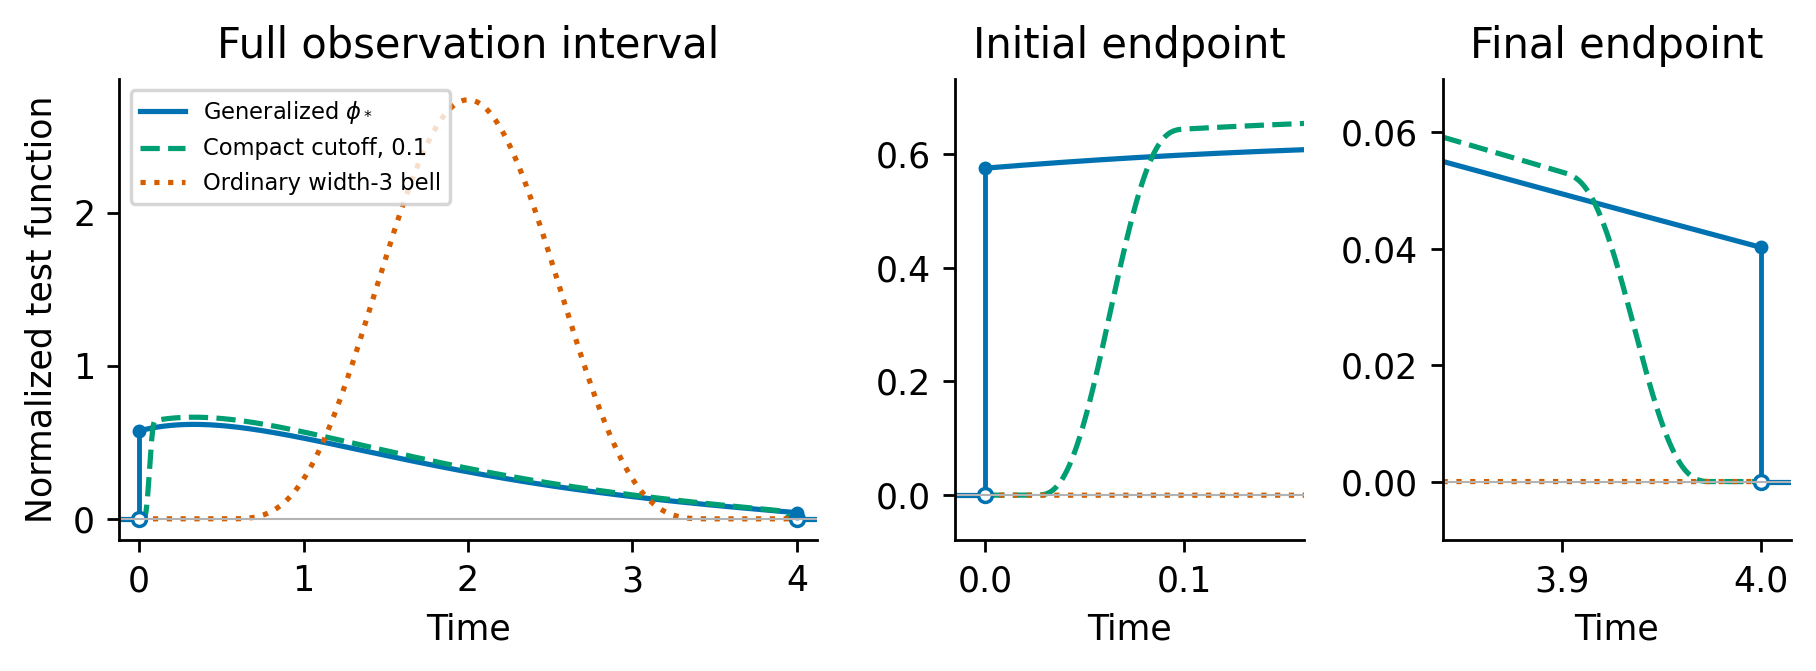
\includegraphics[width=\linewidth,keepaspectratio,alt={Figure 1. Optimal generalized boundary-free test for the scalar ODE x\textquotesingle=ax with a=-1, x(0)=2, T=4 and OU correlation time \textbackslash tau=0.4, its compact cutoff of width 0.1, and an ordinary bell test of width three, all with the same clean-moment normalization. Endpoint panels show the nonzero one-sided traces whose zero extensions produce endpoint atoms.}]{figures/publication/optimal_test_function.png}}
\caption{Optimal generalized boundary-free test for the scalar
ODE \(x'=ax\) with \(a=-1\), \(x(0)=2\), \(T=4\) and OU correlation time
\(\tau=0.4\), its compact cutoff of width 0.1, and an ordinary bell test
of width three, all with the same clean-moment normalization. Endpoint
panels show the nonzero one-sided traces whose zero extensions produce
endpoint atoms.}
\end{figure}

\subsection{Covariance-weighted weak
regression}\label{covariance-weighted-weak-regression}

For tests \(\phi_k\) put \(\lambda_k=\mathcal D^*\phi_k\),
\(D_{kr}=\langle\lambda_k,S_r\rangle\) and
\(\Sigma_{k\ell}=\langle\lambda_k,C\lambda_\ell\rangle\), after removing
exact linear dependencies. If \(D\) has full column rank,
covariance-weighted weak regression has local influence map and
covariance

\[
P=(D^T\Sigma^{-1}D)^{-1}D^T\Sigma^{-1},\qquad
V_K=(D^T\Sigma^{-1}D)^{-1}.
\]

This is the Godambe construction of optimally weighted estimating
equations {[}20{]}, with local information \(D^\top\Sigma^{-1}D\);
WENDy's covariance iteration motivates it {[}4{]}, and WENDy-MLE has the
same leading small-noise map under correctly specified covariance
(S6.3). The first Hermite order of Proposition 4 supplies the weights;
higher orders refine residual covariance at finite amplitude but do not
by themselves remove coefficient bias.

\textbf{Proposition 3 (guarded fixed-family weak GLS).} Fix a finite
deterministic boundary-free test family, a correctly specified
polynomial vector field linear in its coefficients, a known initial
state and a supplied independent-coordinate OU covariance with a known
common correlation time. Suppose that the true coefficient is interior
to a compact box \(\mathcal B\); that clean and nearby pilot
trajectories lie in a common bounded region; that the clean pilot and
final designs have full column rank; that the first-order residual
covariance \(\Sigma_1\) is positive definite; and that the quadrature
weights have bounded total mass, converge to their integrals, and leave
clean and pilot-model numerical defects of order \(o(\epsilon)\) with
the derivative control (G4) of S7.2.

Use a declared pilot family containing the true vector field. Apply
corrected least squares, clip the pilot to its box, evaluate the full
Hermite covariance on its integrated trajectory, and apply the
vanishing-ridge, guarded, box-projected GLS routine of S7.2. Then
\(\widetilde\theta-\theta=O_P(\epsilon)\), the normalized weights
converge, and

\[
\epsilon^{-1}(\widehat\theta_{K,\epsilon}-\theta)\Rightarrow N(0,V_K),\qquad
\epsilon^{-2}\operatorname{Cov}(\widehat\theta_{K,\epsilon})\to V_K,
\]

with uniformly integrable squared scaled errors. The expansion, weight
consistency and integrability are derived, not assumed (proof in S7.2).
For nested dense families satisfying these conditions, the subsequent
family limit attains the bound of Theorem 1.

The archived solvers used for Tables 1--6 differ from this routine: they
use a fixed relative ridge \(\varrho\) and an unbounded final estimate.
For fixed design \(D\), residual shape \(\Sigma_1\) and \(q\) stacked
moments, their regularized linear map is

\[
W_\varrho=[\Sigma_1+\varrho\operatorname{tr}(\Sigma_1)I/q]^{-1},\quad
P_\varrho=(D^\top W_\varrho D)^{-1}D^\top W_\varrho,\quad
V_\varrho=P_\varrho\Sigma_1P_\varrho^\top,
\]

and the exact identity

\[
V_\varrho-V_0=(P_\varrho-P_0)\Sigma_1(P_\varrho-P_0)^\top\succeq0
\]

quantifies the cost of the ridge. On the eight archived 480-window spans
and their endpoint extensions, including Lorenz, the largest relative
RMSE increment is \(6.7\times10^{-15}\) (S7.3), so the ridge has
negligible local cost there. This does not control moments of the
unbounded nonlinear final estimate; Table S8 separates the archived
benchmarks, the constructive estimator and supplied-candidate testing.

\subsection{Extended class with a known initial
state}\label{extended-class-with-a-known-initial-state}

In this subsection \(u\) is known exactly, \(\mathcal I_{\theta\theta}\)
is positive definite, and \(Z(0)=I_d\), \(S(0)=0\). For
\(\phi\in H^1([0,T];\mathbb R^d)\) use the known-initial residual

\[
m_\phi(\theta)=-\int_0^T[\phi'^TY+\phi^Tf_\theta^H(Y)]dt
+\phi(T)^TY(T)-\phi(0)^Tu,
\]

whose first-order influence is
\(L\phi=(-\phi'-J^T\phi)dt+\phi(T)\delta_T\). The initial boundary term
contains the exact state rather than its noisy observation. This
adaptation is due to Brunel et al. {[}5{]}; the result below identifies
its covariance-dual geometry and its relation to an initial-noise
control.

\textbf{Theorem 2 (known-initial extended influence class).} Under these
assumptions,

\[
\overline{L(H^1)}^{\mathcal E}
=\overline{L\{\phi\in H^1:\phi(T)=0\}}^{\mathcal E}
=\mathcal E,
\]

whereas a terminal trace alone preserves the original class:

\[
\overline{L\{\phi\in H^1:\phi(0)=0\}}^{\mathcal E}=\mathcal M.
\]

Adding initial noise controls to the boundary-free class gives the exact
equality

\[
\mathcal M+\{a\delta_0:a\in\mathbb R^d\}=\mathcal E.
\]

In either full closure the sharp normalized influence covariance is
\(\mathcal I_{\theta\theta}^{-1}\), with representative
\(\Lambda_{\mathrm{full}}=C^{-1}S\mathcal I_{\theta\theta}^{-1}\); over
ordinary tests it is an infimum.

\emph{Proof.} For \(g\in\mathcal H\),

\[
\langle g,L\phi\rangle
=\int_0^T\phi^T(g'-Jg)dt+\phi(0)^Tg(0).
\]

If this vanishes for all permitted tests, compact interior tests give
\(g'=Jg\) weakly, so \(g=Zc\). For all \(H^1\) tests, or those with
\(\phi(T)=0\), the initial trace is arbitrary, so \(g(0)=c=0\); the
annihilator is trivial and the closure is \(\mathcal E\). For
\(\phi(0)=0\) every \(Zc\) annihilates the range and there are no other
annihilators, so the closure is \(\mathcal M\) by Proposition 2. For
\(\lambda\in\mathcal E\) define
\(a_j=\langle Z_{\cdot j},\lambda\rangle\), continuous because
\(Z\in\mathcal H\). Since \(Z(0)=I_d\), \(\lambda-a\delta_0\)
annihilates every column of \(Z\) and lies in \(\mathcal M\), proving
the sum identity. Finally
\(\langle\Lambda_{\mathrm{full}},S\rangle=I_p\) and
\(\operatorname{Cov}(\Lambda_{\mathrm{full}})=\mathcal I_{\theta\theta}^{-1}\);
any other normalized influence adds a covariance-orthogonal remainder,
and attainability as an infimum follows as in Theorem 1. \(\square\)

Under the conditions of Proposition 3, correct-covariance GLS on dense
extended spans therefore approaches the full information
\(\mathcal I_{\theta\theta}\). Gains of different endpoint additions can
overlap in finite families. For compact tests with exact Hermite
residual covariance \(\Omega\),
\(\Sigma_0=\operatorname{diag}(\sigma_j^2)\) and
\(\Gamma=\operatorname{Cov}(m_\phi,Y(0)-u)\), the optimal linear control
replaces the residual covariance by

\[
\Omega-\Gamma\Sigma_0^{-1}\Gamma^T.
\]

Only the first Hermite order contributes to \(\Gamma\); in coordinate
\(j\) it is the integral of the linear residual weight against
\(\sigma_j^2e^{-t/\tau_j}\). Under iid sampled noise, compact-test
weights vanish at the initial node and \(\Gamma=0\), so the control is a
genuinely correlated-noise mechanism.

\subsection{Constructive full-library
attainability}\label{constructive-full-library-attainability}

The following procedure estimates every library coefficient; it uses
neither the true support nor any ODE solution. Let \(\mathcal B\) be the
compact coefficient box and use uniform grids with an even number of
intervals. Reflect the linear interpolant of \(Y\) at the endpoints and
smooth it with

\[
\begin{aligned}
K_b(t)&=b^{-1}(315/256)[1-(t/b)^2]_+^4,\quad b=\epsilon^{1/10}/4,\\
w(t)&=[1-((t-T/2)/(T/2-1/2))^2]_+^4.
\end{aligned}
\]

The smoothed proxy \(z\) supplies \(m\) feature tests \(w g_j(z)\) with
analytic derivatives. Their Hermite-corrected weak equations give a
full-library least-squares pilot, clipped to \(\mathcal B\). Append the
cubic splines \(B_3(t/a-j)\), \(a=T/2^k\), \(j=2,\ldots,2^k-2\), where
\(B_3\) is the normalized cardinal cubic spline on \([-2,2]\). Whiten
the combined \(H^1\) Gram matrix, retaining eigenvalues above
\(10^{-10}\epsilon^{1/10}\) times the largest. The exact Hermite
covariance (Proposition 4), evaluated at the proxy and pilot, gives
\(\widehat\Sigma_1=\widehat\Omega/\epsilon^2\). With \(r_k\) retained
scalar tests and \(q_k=d r_k=\dim(\widehat\Sigma_1)\) stacked moments,
add ridge \(\epsilon^2\operatorname{tr}(\widehat\Sigma_1)I_{q_k}/q_k\),
solve corrected GLS and project onto \(\mathcal B\). Relative
minimum-eigenvalue guards use \(10^{-8}\epsilon^2\); singular, nonfinite
or failed calculations return the box midpoint. S8 specifies column
scaling and the covariance guard.

The restriction \(T>1\) only makes the half-unit margins of \(w\)
nonempty; proportional margins and a rescaled kernel work on any
horizon. Write \(\mathcal I_{e,C}\) for the initial-state-adjusted
information of Theorem 1 computed with the covariance \(C\) of \(\eta\).

\textbf{Theorem 3 (constructive attainability under a jet condition).}
Consider an analytic trajectory \(x_0\) of a polynomial ODE on
\([0,T]\), \(T>1\), whose vector field is linear in a polynomial library
\(g_1,\ldots,g_m\) in each of \(d\) equations, with all \(dm\) true
coefficients strictly inside \(\mathcal B\). Observe
\(Y=x_0+\epsilon\eta\) with known independent-coordinate stationary OU
covariance and common correlation time \(\tau>0\). Assume that at some
\(t_*\in[0,T]\)

\[
\det[\partial_t^r g_j(x_0(t_*))]_{r=0,\ldots,m-1;\ j=1,\ldots,m}\ne0.
\]

Let \(h^2=o(\epsilon)\). For each fixed spline level \(k\) the pilot
satisfies \(\widetilde\theta-\theta_0=O_P(\epsilon)\), the normalized
covariance weights are consistent, and

\[
\epsilon^{-1}(\widehat\theta_{k,\epsilon}-\theta_0)\Rightarrow N(0,V_k),\qquad
\epsilon^{-2}E[(\widehat\theta_{k,\epsilon}-\theta_0)(\widehat\theta_{k,\epsilon}-\theta_0)^\top]\to V_k,
\]

with uniformly integrable squared scaled errors. Moreover
\(V_k\to\mathcal I_{e,C}^{-1}\) as \(k\to\infty\) after the fixed-level
small-noise limit.

The jet determinant is the Wronskian of the library functions along the
trajectory. Since \(t\mapsto g_j(x_0(t))\) are analytic, it is nonzero
at some \(t_*\) if and only if these functions are linearly independent
on \([0,T]\); the condition is therefore identifiability of the library
along the observed trajectory rather than an additional restriction. The
procedure does not use the initial state, so it targets the
boundary-free bound \(\mathcal I_{e,C}^{-1}\) even when \(u\) is known.
Theorem 2 shows that adding initial-trace tests then enlarges the class
to full information; extending the constructive proof to such tests is
left open.

S8.1 proves the theorem, including rank, weight consistency and moment
control. S8.2 verifies the jet condition for Van der Pol with the full
eighteen-coefficient cubic library and \(u=(2,0)\): the determinant
equals \(-65265167726360395776\).

\textbf{Relation to existing efficiency results.} Generalized profiling
is asymptotically efficient for independent errors observed at an
increasing number of points {[}18{]}; direct integral estimators attain
the root-\(n\) rate in that experiment {[}15, 16{]}, and one-step
likelihood refinement of such a pilot reaches efficiency {[}19{]}.
Theorem 3 differs in three respects. First, the experiment has a fixed
horizon and physical OU error, so information does not grow with the
number of samples (Lemma 1) and the relevant limit is small noise.
Second, the bound is attained by estimating equations alone, without
integrating the ODE as likelihood refinement does. Third, every library
coefficient is estimated without a supplied support, and identifiability
of the weak equations reduces to one jet determinant that can be checked
by exact symbolic computation. The price is the absence of rates: the
theorem holds at each fixed spline level and then in the dense-span
limit, and it does not concern finite-noise Wald calibration.

\section{Exact polynomial weak-residual
covariance}\label{exact-polynomial-weak-residual-covariance}

\subsection{Finite Hermite
expansion}\label{finite-hermite-expansion}

Assume a common \(\tau\) for independent coordinates and set
\(v_j=\sigma_j^2\). Define \(H_0(z;v)=1\), \(H_1(z;v)=z\),
\(H_{q+1}(z;v)=zH_q(z;v)-qvH_{q-1}(z;v)\) and corrected monomials
\(\widetilde\vartheta_\beta(y)=\prod_jH_{\beta_j}(y_j;v_j)\), whose
expectation given \(x\) is \(x^\beta\) {[}27{]}. The continuum residual
\(r_{ki}=b_{ki}-(G\xi^*)_{ki}\) then expands as

\[
r_{ki}=\sum_{1\leq|\alpha|\leq p_*}\int_0^Tc_{ki,\alpha}(t)H_\alpha(\eta_C(t);v)dt,
\qquad
c_{ki,\alpha}=-\mathbf1_{\{\alpha=e_i\}}\phi'_k
-\phi_k\frac{\partial^\alpha f_i(x)}{\alpha!},
\]

where \(p_*\geq1\) is the maximum degree and
\(H_\alpha=\prod_jH_{\alpha_j}\). Response and feature perturbations
share these coefficients and keep their cross-covariance.

\textbf{Proposition 4 (exact covariance).} Under these assumptions,

\[
\operatorname{Cov}(r_{ki},r_{\ell m})=
\sum_{1\leq|\alpha|\leq p_*}\alpha!\prod_jv_j^{\alpha_j}
\int_0^T\int_0^Tc_{ki,\alpha}(s)c_{\ell m,\alpha}(t)
e^{-|\alpha||s-t|/\tau}\,ds\,dt.
\]

\textbf{Proof.} The generating function \(\exp(az-va^2/2)\) gives
\(E[H_q(U;v)H_r(V;v)]=\mathbf1_{q=r}q!v^q\rho^q\) for jointly Gaussian
variables of variance \(v\) and correlation \(\rho\), the Hermite form
of classical Gaussian moment identities {[}36{]}. Coordinate
independence gives orthogonality between multi-indices and the factor
\(\alpha!\prod_jv_j^{\alpha_j}\). Substitute \(\rho=e^{-|s-t|/\tau}\)
and integrate. \(\square\)

Order \(q\) has correlation time \(\tau/q\) and need not be negligible
at moderate amplitude. Different windows and equations remain correlated
despite independent sensor coordinates. The covariance is exact at the
clean trajectory and true coefficients; plug-in estimates add an
approximation.

\subsection{Implementation and covariance
misspecification}\label{implementation-and-covariance-misspecification}

The Hermite sum is evaluated on the grid in linear time without a dense
temporal matrix (S6.4, which also treats incorrectly corrected raw
features). Under misspecified temporal weights \(W\) the leading
covariance is \(P_W\Sigma_{\mathrm{true},1}P_W^\top\), and wrong
correction variances can also shift the moment mean. Sensitivity to
supplied and fitted correlation times is reported in S5.4.

\section{Numerical benchmarks}\label{numerical-benchmarks}

All benchmarks use fully observed polynomial systems, supplied structure
and sensor covariance, and archived paired observations; covariance
pilots never receive the generating coefficients. Relative errors divide
the coefficient error norm by the norm of the true coefficient vector.
Protocols, seed ranges and fingerprints are in S2--S5.

Three test families are compared. \emph{Interior windows} are compactly
supported smooth bumps at prescribed multiscale positions and widths;
they span boundary-free influences. \emph{Universal endpoint tests} add,
without using the ODE, twelve endpoint half-bumps (bumps centred at
\(0\) or \(T\) and truncated there, with full widths
\(3,1.5,\ldots,0.09375\)), which have nonzero traces, together with the
\(d\) initial controls \(Y(0)-u\). \emph{Model-adjoint tests} are
obtained by integrating the adjoint equation at the pilot so that their
influences contain the efficient score directions of Theorem 2; they
serve as an implementation check. In Sections 7.1--7.4, covariance
weights come from a bounded 30-window pilot fit integrated from the
known initial state; the constructive estimator of Section 7.6
integrates no ODE.

\subsection{Information cost and finite-span
efficiency}\label{information-cost-and-finite-span-efficiency}

For Van der Pol we fit four coefficients in \(x'=a v\),
\(v'=b x+c v+d_3x^2v\), with truth \((1,-1,1,-1)\), \(u=(2,0)\),
\(T=20\), \(h=0.005\) and OU correlation time 0.3. At 5\% noise the
known-initial local RMSE reference is 0.013093 and the boundary-free
reference is 0.016904, a 29\% cost. Both scale linearly with noise
amplitude.

\begin{center}
\begin{minipage}{\linewidth}
Table 1. Oracle Gaussian influence RMSE under OU noise at 5\%. Both
columns use the same test span and clean design and differ only in the
covariance used for GLS weights.

\small\setlength{\tabcolsep}{3pt}
\begin{tabular}{@{}
  >{\raggedleft\arraybackslash}p{(\linewidth - 8\tabcolsep) * \real{0.2000}}
  >{\raggedleft\arraybackslash}p{(\linewidth - 8\tabcolsep) * \real{0.2000}}
  >{\raggedleft\arraybackslash}p{(\linewidth - 8\tabcolsep) * \real{0.2000}}
  >{\raggedleft\arraybackslash}p{(\linewidth - 8\tabcolsep) * \real{0.2000}}
  >{\raggedleft\arraybackslash}p{(\linewidth - 8\tabcolsep) * \real{0.2000}}@{}}
\toprule\noalign{}
\begin{minipage}[b]{\linewidth}\raggedleft
Prescribed windows
\end{minipage} & \begin{minipage}[b]{\linewidth}\raggedleft
Retained tests
\end{minipage} & \begin{minipage}[b]{\linewidth}\raggedleft
OU-weight RMSE
\end{minipage} & \begin{minipage}[b]{\linewidth}\raggedleft
iid-weight RMSE
\end{minipage} & \begin{minipage}[b]{\linewidth}\raggedleft
OU RMSE / class reference
\end{minipage} \\
\midrule\noalign{}
30 & 30 & 0.019605 & 0.020296 & 1.1597 \\
120 & 120 & 0.017043 & 0.017839 & 1.0082 \\
480 & 479 & 0.016938 & 0.017734 & 1.0020 \\
\bottomrule
\end{tabular}
\end{minipage}
\end{center}

Rich spans produce most of the improvement: 480-window OU GLS is within
0.2\% of the boundary-free reference, whereas iid weights keep a gap of
about 5\%.

\begin{center}
\begin{minipage}{\linewidth}
Table 2. Van der Pol on 2000 paths at 0.5\% noise. The local reference
is the leading Gaussian influence RMSE; all paths are retained.

\small\setlength{\tabcolsep}{3pt}
\begin{tabular}{@{}
  >{\raggedright\arraybackslash}p{(\linewidth - 8\tabcolsep) * \real{0.1579}}
  >{\raggedleft\arraybackslash}p{(\linewidth - 8\tabcolsep) * \real{0.2105}}
  >{\raggedleft\arraybackslash}p{(\linewidth - 8\tabcolsep) * \real{0.2105}}
  >{\raggedleft\arraybackslash}p{(\linewidth - 8\tabcolsep) * \real{0.2105}}
  >{\raggedleft\arraybackslash}p{(\linewidth - 8\tabcolsep) * \real{0.2105}}@{}}
\toprule\noalign{}
\begin{minipage}[b]{\linewidth}\raggedright
Estimator
\end{minipage} & \begin{minipage}[b]{\linewidth}\raggedleft
RMSE (95\% interval)
\end{minipage} & \begin{minipage}[b]{\linewidth}\raggedleft
Bias
\end{minipage} & \begin{minipage}[b]{\linewidth}\raggedleft
Dispersion
\end{minipage} & \begin{minipage}[b]{\linewidth}\raggedleft
Local reference
\end{minipage} \\
\midrule\noalign{}
One step, known initial & 0.001301 {[}0.001269, 0.001332{]} & 0.000085 &
0.001298 & 0.001309 \\
One step, unknown initial & 0.001838 {[}0.001790, 0.001887{]} & 0.000469
& 0.001777 & 0.001690 \\
Three steps, unknown initial & 0.001669 {[}0.001630, 0.001708{]} &
0.000068 & 0.001668 & 0.001690 \\
Weak GLS, OU & 0.001685 {[}0.001645, 0.001723{]} & 0.000083 & 0.001683 &
0.001690 \\
Weak GLS, iid & 0.001759 {[}0.001718, 0.001801{]} & 0.000103 & 0.001756
& 0.001690 \\
\bottomrule
\end{tabular}
\end{minipage}
\end{center}

Weak GLS uses 480 prescribed windows; likelihood refinements use exact
OU innovations and analytic sensitivities. The paired iid-minus-OU RMSE
difference is 0.00007426 (95\% bootstrap interval {[}0.00005576,
0.00009327{]}), a 4.22\% benefit of temporal weighting. One
unknown-initial scoring step retains nonlinear initialization bias;
three steps reach the nuisance-adjusted reference. The known-initial
estimate is more accurate because it uses the information that compact
tests discard.

\begin{figure}[p]
\centering
\pandocbounded{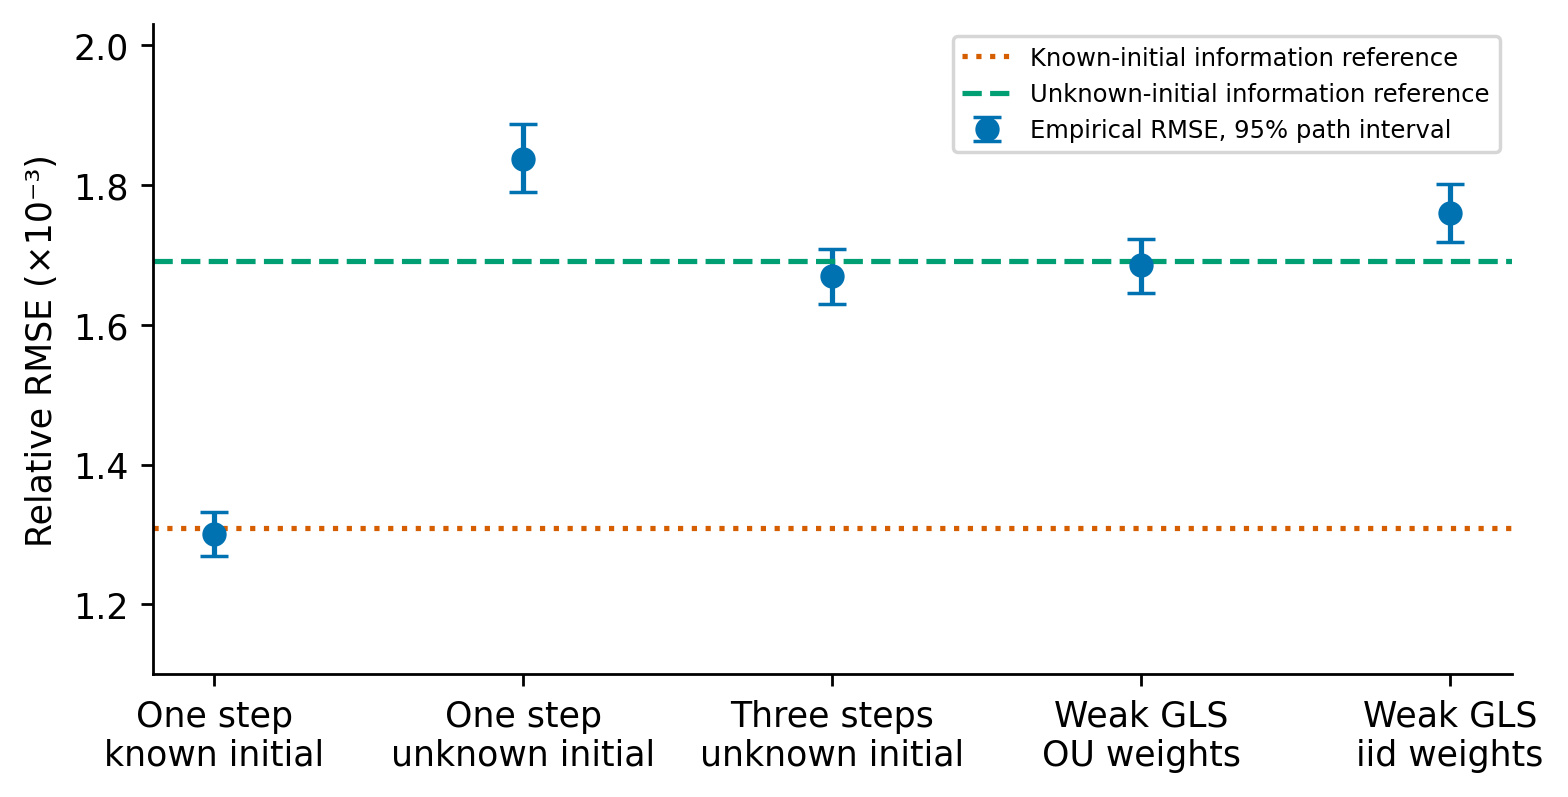
\includegraphics[width=\linewidth,keepaspectratio,alt={Figure 2. Van der Pol on 2000 shared paths at 0.5\% noise: one scoring step with known initial state, one or three joint steps with unknown initial state, and weak GLS with OU or iid weights. Whiskers are 95\% bootstrap intervals for RMSE over independent paths. Dotted and dashed lines mark the known-initial and unknown-initial local information references.}]{figures/publication/likelihood_comparison.png}}
\caption{Van der Pol on 2000 shared paths at 0.5\% noise: one
scoring step with known initial state, one or three joint steps with
unknown initial state, and weak GLS with OU or iid weights. Whiskers are
95\% bootstrap intervals for RMSE over independent paths. Dotted and
dashed lines mark the known-initial and unknown-initial local
information references.}
\end{figure}

\subsection{Recovery with universal endpoint
tests}\label{recovery-with-universal-endpoint-tests}

With known \(u\), the universal family uses the residual \(m_\phi\) of
Section 5.5 with 480 interior windows, twelve endpoint half-bumps and
the initial controls. The relative success criteria (at least 50\%
recovery of the weak-to-scoring gap; model-adjoint RMSE within 5\% of
scoring) replaced an unsuitable absolute screen threshold before any new
endpoint outcomes were inspected; S5.5 records the amendment and the
quadrature checks.

\begin{center}
\begin{minipage}{\linewidth}
Table 3. Known-initial endpoint confirmation on 1968 paired Van der Pol
paths at 0.5\% noise. The likelihood reference is one known-initial
Fisher-scoring step.

\small\setlength{\tabcolsep}{3pt}
\begin{tabular}{@{}lrrr@{}}
\toprule\noalign{}
Method & RMSE & Bias norm & Dispersion \\
\midrule\noalign{}
Boundary-free, 480 & 0.00168754 & 0.00008679 & 0.00168531 \\
Universal endpoints & 0.00130936 & 0.00007049 & 0.00130746 \\
Model-adjoint endpoints & 0.00129741 & 0.00006771 & 0.00129564 \\
Known-initial scoring & 0.00129800 & 0.00008753 & 0.00129505 \\
\bottomrule
\end{tabular}
\end{minipage}
\end{center}

Universal endpoints recover 97.1\% of the gap (paired interval
95.5--98.6\%) and lie 0.88\% above scoring; model-adjoint tests match
scoring, confirming the implementation.

\begin{figure}[p]
\centering
\pandocbounded{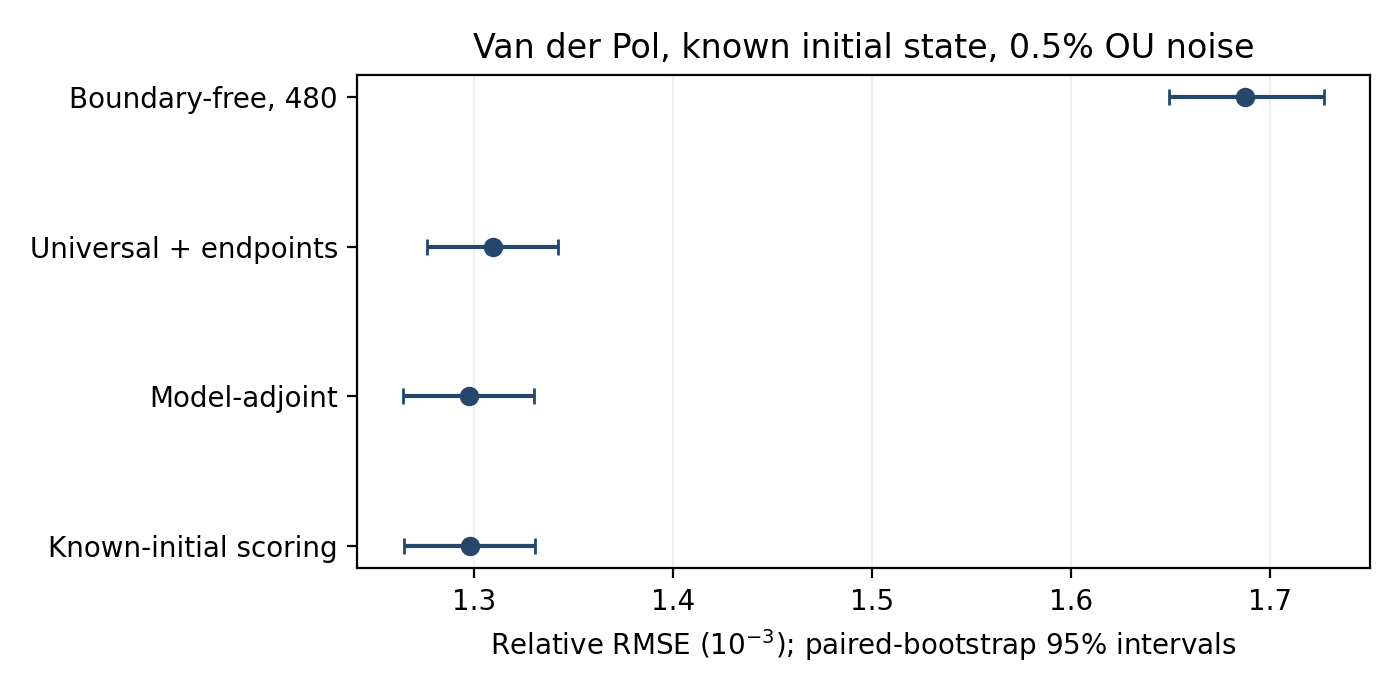
\includegraphics[width=\linewidth,keepaspectratio,alt={Figure 3. Known-initial information recovery on 1968 paired Van der Pol records at 0.5\% OU noise. Whiskers are 95\% RMSE intervals from shared record bootstrap resamples. Universal time-only endpoint tests recover 97.1\% of the weak-to-scoring gap; model-adjoint tests check score realization.}]{figures/publication/endpoint_confirmation.png}}
\caption{Known-initial information recovery on 1968 paired Van
der Pol records at 0.5\% OU noise. Whiskers are 95\% RMSE intervals from
shared record bootstrap resamples. Universal time-only endpoint tests
recover 97.1\% of the weak-to-scoring gap; model-adjoint tests check
score realization.}
\end{figure}

\subsection{Attribution to initial
traces}\label{attribution-to-initial-traces}

The 500-path ablation holds Simpson quadrature and the covariance pilot
fixed and adds one endpoint component at a time to a matched
boundary-free branch.

\begin{center}
\begin{minipage}{\linewidth}
Table 4. Endpoint-component ablation on 500 paired paths at 0.5\% noise.
Gap closure is measured between the matched boundary-free branch and
known-initial scoring; intervals resample common record indices.

\small\setlength{\tabcolsep}{3pt}
\begin{tabular}{@{}lrrr@{}}
\toprule\noalign{}
Added component & RMSE & Gap closed & Paired 95\% interval \\
\midrule\noalign{}
Initial half-windows & 0.00132445 & 98.9\% & {[}95.1\%; 102.7\%{]} \\
Terminal half-windows & 0.00164493 & -0.3\% & {[}-1.8\%; 1.2\%{]} \\
Initial controls only & 0.00159795 & 14.3\% & {[}7.0\%; 21.4\%{]} \\
All components & 0.00132453 & 98.9\% & {[}95.1\%; 102.6\%{]} \\
Matched boundary-free & 0.00164395 & 0\% & --- \\
Known-initial scoring & 0.00132100 & 100\% & --- \\
\bottomrule
\end{tabular}
\end{minipage}
\end{center}

Initial traces alone recover essentially the entire gap, as Theorem 2
predicts and as in the Brunel adaptation; terminal traces recover
nothing, consistent with the unchanged class. Initial controls alone
recover 14.3\%, but add no resolved gain to initial traces: the
all-minus-initial RMSE difference is \(7.46\times10^{-8}\) with paired
interval \([-7.18\times10^{-7},8.55\times10^{-7}]\). Component
contributions overlap and are not additive.

\begin{figure}[p]
\centering
\pandocbounded{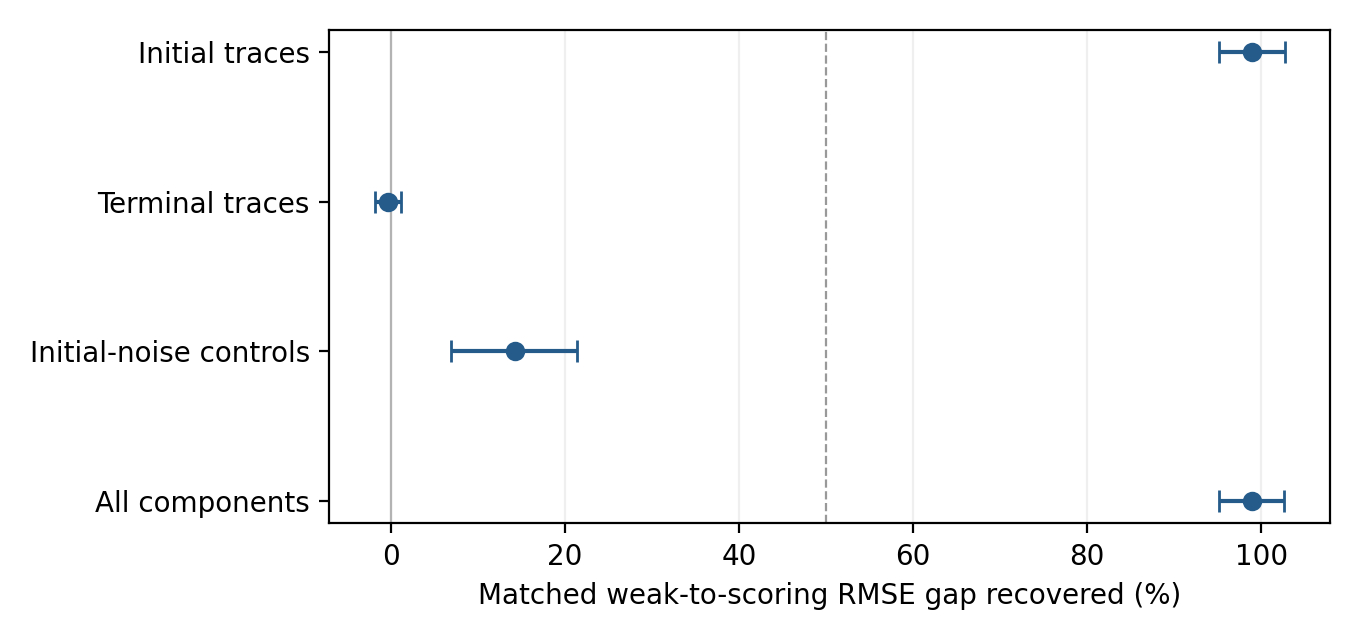
\includegraphics[width=\linewidth,keepaspectratio,alt={Figure 4. Paired endpoint-component attribution on 500 Van der Pol records. Whiskers show 95\% bootstrap intervals for the fraction of the matched weak-to-scoring RMSE gap recovered; the dashed line marks the prespecified 50\% rule.}]{figures/publication/endpoint_ablation.png}}
\caption{Paired endpoint-component attribution on 500 Van der
Pol records. Whiskers show 95\% bootstrap intervals for the fraction of
the matched weak-to-scoring RMSE gap recovered; the dashed line marks
the prespecified 50\% rule.}
\end{figure}

\subsection{Moderate noise and
Lorenz}\label{moderate-noise-and-lorenz}

At 5\% noise the Van der Pol comparison uses all 128 matched paths, the
same feasible pilot and full nonlinear likelihood fits with exact OU
innovations.

\begin{center}
\begin{minipage}{\linewidth}
Table 5. Moderate-noise endpoint comparison on 128 paired Van der Pol
paths at 5\% noise.

\small\setlength{\tabcolsep}{3pt}
\begin{tabular}{@{}lrrr@{}}
\toprule\noalign{}
Method & RMSE & Bias norm & Dispersion \\
\midrule\noalign{}
Matched boundary-free & 0.0255965 & 0.0081646 & 0.0242594 \\
Universal endpoints & 0.0218790 & 0.0056954 & 0.0211247 \\
Known-initial MLE & 0.0142088 & 0.0007255 & 0.0141902 \\
Unknown-initial MLE & 0.0171952 & 0.0006504 & 0.0171829 \\
\bottomrule
\end{tabular}
\end{minipage}
\end{center}

Universal endpoints recover only 32.6\% of the gap (18.3--45.8\%),
failing the 50\% criterion. Their dispersion 0.021125 exceeds the
clean-design first-order and full-Hermite references 0.013094 and
0.013636, so at this amplitude finite-noise design, pilot and fitting
effects dominate the restored local geometry. A matched comparison with
the authors' WENDy implementation is in S5.3.

For Lorenz we fit \((s,r,b)=(10,28,8/3)\) in the supplied physical
structure, with \(u=(1,1,1)\), \(T=4\), \(h=0.001\), OU correlation time
0.1 and 0.5\% coordinate noise. The local relative RMSE reference is
0.000411 with unknown and 0.000209 with known initial state, almost a
factor two.

\begin{center}
\begin{minipage}{\linewidth}
Table 6. Lorenz endpoint confirmation on 256 paired paths at 0.5\%
noise.

\small\setlength{\tabcolsep}{3pt}
\begin{tabular}{@{}lrrr@{}}
\toprule\noalign{}
Method & RMSE & Bias norm & Dispersion \\
\midrule\noalign{}
Matched boundary-free & 0.00040994 & 0.00002170 & 0.00040936 \\
Universal endpoints & 0.00021686 & 0.00002153 & 0.00021579 \\
Known-initial MLE & 0.00020784 & 0.00002355 & 0.00020650 \\
\bottomrule
\end{tabular}
\end{minipage}
\end{center}

All 256 paths are retained. Universal endpoints recover 95.5\% of the
gap (92.8--98.0\%); their dispersion is close to the full-Hermite
reference 0.00020926.

\subsection{Direction-specific information
cost}\label{direction-specific-information-cost}

For the negative cubic perturbation \(\delta x^3\) in the second Van der
Pol equation, profiling the seventeen other library coefficients gives
full-information and boundary-free two-point reference magnitudes
0.01928 and 0.01941 at 0.5\% noise. The initial-state cost in this
direction is only 0.68\%, far below the aggregate coefficient cost.
Supplied-candidate Wald testing and sparse selection are compared in S3,
S4 and S9.

\subsection{The constructive estimator against its finite-span
reference}\label{the-constructive-estimator-against-its-finite-span-reference}

The interior proxy smoothing bias is \(O(b^2)=O(\epsilon^{1/5})\) (Lemma
S8.A), so the instruments converge slowly, although the clean weak
identity still gives \(\widetilde\theta-\theta_0=O_P(\epsilon)\). The
problem is ill-conditioned: the clean raw Gram matrix has minimum
eigenvalue \(6.07\times10^{-10}\) and condition number at least
\(7.1\times10^9\), and the column-scaled GLS normal matrix has condition
number \(1.40\times10^6\). Positivity at a fixed level suffices for
Theorem 3, but its constants depend on these gaps.

The estimator uses nine smoothed-data feature instruments and 125 cubic
splines. The deterministic limiting covariance for this 134-test span
has \(\sqrt{\operatorname{tr}V_k}=9.8144\), computed without ridge or
truncation; halving the finest grid changes it by \(4.7\times10^{-8}\)
relatively. It concerns all eighteen coefficients, unlike the
four-coefficient benchmarks above.

\begin{center}
\begin{minipage}{\linewidth}
Table 7. Constructive full-library estimator on 100 independent paths
per amplitude. Intervals are pointwise and resample archived coefficient
errors 10,000 times.

\small\setlength{\tabcolsep}{3pt}
\begin{tabular}{@{}
  >{\raggedleft\arraybackslash}p{(\linewidth - 6\tabcolsep) * \real{0.2500}}
  >{\raggedleft\arraybackslash}p{(\linewidth - 6\tabcolsep) * \real{0.2500}}
  >{\raggedleft\arraybackslash}p{(\linewidth - 6\tabcolsep) * \real{0.2500}}
  >{\raggedleft\arraybackslash}p{(\linewidth - 6\tabcolsep) * \real{0.2500}}@{}}
\toprule\noalign{}
\begin{minipage}[b]{\linewidth}\raggedleft
Noise
\end{minipage} & \begin{minipage}[b]{\linewidth}\raggedleft
RMSE/\(\epsilon\)
\end{minipage} & \begin{minipage}[b]{\linewidth}\raggedleft
RMSE/\((\epsilon\sqrt{\operatorname{tr}V_k})\)
\end{minipage} & \begin{minipage}[b]{\linewidth}\raggedleft
95\% interval for ratio
\end{minipage} \\
\midrule\noalign{}
5\% & 11.6265 & 1.1846 & 1.1140--1.2563 \\
0.5\% & 10.3505 & 1.0546 & 0.9883--1.1202 \\
0.1\% & 9.9850 & 1.0174 & 0.9452--1.0885 \\
0.05\% & 9.5899 & 0.9771 & 0.8994--1.0528 \\
0.01\% & 9.3516 & 0.9528 & 0.8891--1.0147 \\
\bottomrule
\end{tabular}
\end{minipage}
\end{center}

The four lower-noise intervals include one; the 5\% interval lies above
it. No guard fallback or final clipping occurred on the 500 paths. At
0.01\% noise the spectral cutoff retained 133 tests in 65 fits and 132
in 35, so the finite-amplitude estimator does not use exactly the
134-test reference span, and a ratio slightly below one is not excluded.
With 100 paths per level, the apparent downward trend is not resolved;
the ratios show compatibility with the limiting reference rather than
numerical proof of attainment. At 5\% noise the eighteen-coefficient
RMSE is 0.5813 (root-mean-square coordinate error 0.1370): the
construction is an asymptotic witness, not a recommended moderate-noise
method. S9.2 records matrix checks and covariance diagnostics.

\section{Discussion and
limitations}\label{discussion-and-limitations}

Boundary-free weak equations retain exactly the local information
available when the initial state is a nuisance parameter. When the state
is known, the cost is 29\% of the aggregate RMSE reference for Van der
Pol and almost a factor two for Lorenz, but it is direction specific:
only 0.68\% for a cubic-term perturbation. The theoretical contributions
are the exact adjoint-range identities and the constructive
attainability result; the projection formulas are classical and the
trace remedy is Brunel's.

In practice, when the initial state is known and errors are temporally
correlated, test functions with a nonzero initial trace should be used.
Time-only endpoint half-bumps recover 97.1\% of the gap for Van der Pol
and 95.5\% for Lorenz at small noise, and the ablation attributes
essentially all of this to initial traces. The correlated-noise initial
control helps on its own (14.3\%) but not in addition to traces. Correct
OU weighting adds a smaller gain of about 4\%.

The limitations are substantial. At 5\% Van der Pol noise only 32.6\% of
the likelihood gap is recovered, likelihood remains more accurate than
the weak estimators, and the constructive full-library estimator is
imprecise. The covariance weights of the endpoint benchmark estimators
in Section 7 still require an integrated pilot model, and no
computational advantage has been demonstrated. Theorem 3 gives
sequential limits without joint span--noise rates, and exact residual
covariance does not yield exact finite-noise estimator variance when
weights and designs depend on the record. The numerical evidence covers
two synthetic systems with supplied covariance and full observation;
unknown covariance, heterogeneous states, partial observation, process
noise and real data require further work. Independent-record GMM,
fission and cross-fitting are preserved in a separate research archive
and lie outside the main claims.

\section*{Data availability}\label{data-availability}

The current code and synthetic-data archive, v1.3.2, is publicly
available in the
\href{https://github.com/malyshevdanil/wsindy-information-limits/tree/v1.3.2}{versioned
reproducibility repository}. Configurations, seed ranges, source
fingerprints, coefficient estimates, covariance summaries and SHA256
manifests permit exact input reconstruction and paired audit. Full
synthetic time series are regenerated from the prespecified seed
protocol. Pinned download specifications retrieve original author
sources. The separate research archive preserves earlier extensions. The
\href{https://doi.org/10.5281/zenodo.23313935}{preceding v1.2.0
snapshot} remains unchanged. No external experimental dataset is used.

\section*{Declaration of generative AI and AI-assisted technologies}\label{declaration-of-generative-ai-and-ai-assisted-technologies}

Codex assisted with research code, literature searches,
Russian-to-English translation, and mathematical derivations and proof
development. The author verified the results and takes full
responsibility for the manuscript.

\subsection*{References}\label{references}
\addcontentsline{toc}{subsection}{References}

\protect\phantomsection\label{refs}
\begin{CSLReferences}{0}{0}
\bibitem[\citeproctext]{ref-schaeffer2017}
\CSLLeftMargin{{[}1{]} }%
\CSLRightInline{Schaeffer H, McCalla SG. Sparse model selection via
integral terms. \emph{Physical Review E} 96 (2017) 023302.
\url{https://doi.org/10.1103/PhysRevE.96.023302}.}

\bibitem[\citeproctext]{ref-messenger2021}
\CSLLeftMargin{{[}2{]} }%
\CSLRightInline{Messenger DA, Bortz DM. Weak {SINDy}: Galerkin-based
data-driven model selection. \emph{Multiscale Modeling and Simulation}
19 (2021) 1474--1497. \url{https://doi.org/10.1137/20M1343166}.}

\bibitem[\citeproctext]{ref-reinbold2020}
\CSLLeftMargin{{[}3{]} }%
\CSLRightInline{Reinbold PAK, Gurevich DR, Grigoriev RO. Using noisy or
incomplete data to discover models of spatiotemporal dynamics.
\emph{Physical Review E} 101 (2020) 010203.
\url{https://doi.org/10.1103/PhysRevE.101.010203}.}

\bibitem[\citeproctext]{ref-bortz2023}
\CSLLeftMargin{{[}4{]} }%
\CSLRightInline{Bortz DM, Messenger DA, Dukic V. Direct estimation of
parameters in {ODE} models using {WENDy}: Weak-form estimation of
nonlinear dynamics. \emph{Bulletin of Mathematical Biology} 85 (2023)
110. \url{https://doi.org/10.1007/s11538-023-01208-6}.}

\bibitem[\citeproctext]{ref-brunel2014}
\CSLLeftMargin{{[}5{]} }%
\CSLRightInline{{Brunel NJ-B, Clairon Q, d'Alche-Buc F}. Parametric
estimation of ordinary differential equations with orthogonality
conditions. \emph{Journal of the American Statistical Association} 109
(2014) 173--185. \url{https://doi.org/10.1080/01621459.2013.841583}.}

\bibitem[\citeproctext]{ref-heitzman2026}
\CSLLeftMargin{{[}6{]} }%
\CSLRightInline{Heitzman-Breen N, Dukic V, Bortz DM. A practical
identifiability criterion leveraging weak-form parameter estimation.
\emph{Bulletin of Mathematical Biology} 88 (2026) 70.
\url{https://doi.org/10.1007/s11538-026-01639-x}.}

\bibitem[\citeproctext]{ref-stein1999}
\CSLLeftMargin{{[}7{]} }%
\CSLRightInline{Stein ML. Interpolation of spatial data: Some theory for
kriging. Springer (1999)
\url{https://doi.org/10.1007/978-1-4612-1494-6}.}

\bibitem[\citeproctext]{ref-ying1991}
\CSLLeftMargin{{[}8{]} }%
\CSLRightInline{Ying Z. Asymptotic properties of a maximum likelihood
estimator with data from a {G}aussian process. \emph{Journal of
Multivariate Analysis} 36 (1991) 280--296.
\url{https://doi.org/10.1016/0047-259X(91)90062-7}.}

\bibitem[\citeproctext]{ref-zhang2004}
\CSLLeftMargin{{[}9{]} }%
\CSLRightInline{Zhang H. Inconsistent estimation and asymptotically
equal interpolations in model-based geostatistics. \emph{Journal of the
American Statistical Association} 99 (2004) 250--261.
\url{https://doi.org/10.1198/016214504000000241}.}

\bibitem[\citeproctext]{ref-bickel1993}
\CSLLeftMargin{{[}10{]} }%
\CSLRightInline{Bickel PJ, Klaassen CAJ, Ritov Y, Wellner JA.
\href{https://faculty.washington.edu/jonw/RESEARCH/BOOKS/book3.html}{Efficient
and adaptive estimation for semiparametric models}. Johns Hopkins
University Press (1993).}

\bibitem[\citeproctext]{ref-vandervaart1998}
\CSLLeftMargin{{[}11{]} }%
\CSLRightInline{{van der Vaart AW}. Asymptotic statistics. Cambridge
University Press (1998) \url{https://doi.org/10.1017/CBO9780511802256}.}

\bibitem[\citeproctext]{ref-varah1982}
\CSLLeftMargin{{[}12{]} }%
\CSLRightInline{Varah JM. A spline least squares method for numerical
parameter estimation in differential equations. \emph{SIAM Journal on
Scientific and Statistical Computing} 3 (1982) 28--46.
\url{https://doi.org/10.1137/0903003}.}

\bibitem[\citeproctext]{ref-brunel2008}
\CSLLeftMargin{{[}13{]} }%
\CSLRightInline{Brunel NJ-B. Parameter estimation of {ODE}'s via
nonparametric estimators. \emph{Electronic Journal of Statistics} 2
(2008) 1242--1267. \url{https://doi.org/10.1214/07-EJS132}.}

\bibitem[\citeproctext]{ref-liang2008}
\CSLLeftMargin{{[}14{]} }%
\CSLRightInline{Liang H, Wu H. Parameter estimation for differential
equation models using a framework of measurement error in regression
models. \emph{Journal of the American Statistical Association} 103
(2008) 1570--1583. \url{https://doi.org/10.1198/016214508000000797}.}

\bibitem[\citeproctext]{ref-gugushvili2012}
\CSLLeftMargin{{[}15{]} }%
\CSLRightInline{Gugushvili S, Klaassen CAJ. \(\sqrt{n}\)-consistent
parameter estimation for systems of ordinary differential equations:
Bypassing numerical integration via smoothing. \emph{Bernoulli} 18
(2012) 1061--1098. \url{https://doi.org/10.3150/11-BEJ362}.}

\bibitem[\citeproctext]{ref-dattner2015}
\CSLLeftMargin{{[}16{]} }%
\CSLRightInline{Dattner I, Klaassen CAJ. Optimal rate of direct
estimators in systems of ordinary differential equations linear in
functions of the parameters. \emph{Electronic Journal of Statistics} 9
(2015) 1939--1973. \url{https://doi.org/10.1214/15-EJS1053}.}

\bibitem[\citeproctext]{ref-ramsay2007}
\CSLLeftMargin{{[}17{]} }%
\CSLRightInline{Ramsay JO, Hooker G, Campbell D, Cao J. Parameter
estimation for differential equations: A generalized smoothing approach.
\emph{Journal of the Royal Statistical Society: Series B} 69 (2007)
741--796. \url{https://doi.org/10.1111/j.1467-9868.2007.00610.x}.}

\bibitem[\citeproctext]{ref-qi2010}
\CSLLeftMargin{{[}18{]} }%
\CSLRightInline{Qi X, Zhao H. Asymptotic efficiency and finite-sample
properties of the generalized profiling estimation of parameters in
ordinary differential equations. \emph{The Annals of Statistics} 38
(2010) 435--481. \url{https://doi.org/10.1214/09-AOS724}.}

\bibitem[\citeproctext]{ref-dattner2018}
\CSLLeftMargin{{[}19{]} }%
\CSLRightInline{Dattner I, Gugushvili S. Application of one-step method
to parameter estimation in {ODE} models. \emph{Statistica Neerlandica}
72 (2018) 126--156. \url{https://doi.org/10.1111/stan.12124}.}

\bibitem[\citeproctext]{ref-godambe1960}
\CSLLeftMargin{{[}20{]} }%
\CSLRightInline{Godambe VP. An optimum property of regular maximum
likelihood estimation. \emph{The Annals of Mathematical Statistics} 31
(1960) 1208--1211. \url{https://doi.org/10.1214/aoms/1177705693}.}

\bibitem[\citeproctext]{ref-dette2016}
\CSLLeftMargin{{[}21{]} }%
\CSLRightInline{Dette H, Pepelyshev A, Zhigljavsky A. Optimal designs in
regression with correlated errors. \emph{The Annals of Statistics} 44
(2016) 113--152. \url{https://doi.org/10.1214/15-AOS1361}.}

\bibitem[\citeproctext]{ref-dette2017}
\CSLLeftMargin{{[}22{]} }%
\CSLRightInline{Dette H, Konstantinou M, Zhigljavsky A. A new approach
to optimal designs for correlated observations. \emph{The Annals of
Statistics} 45 (2017) 1579--1608.
\url{https://doi.org/10.1214/16-AOS1500}.}

\bibitem[\citeproctext]{ref-brunton2016}
\CSLLeftMargin{{[}23{]} }%
\CSLRightInline{Brunton SL, Proctor JL, Kutz JN. Discovering governing
equations from data by sparse identification of nonlinear dynamical
systems. \emph{Proceedings of the National Academy of Sciences} 113
(2016) 3932--3937. \url{https://doi.org/10.1073/pnas.1517384113}.}

\bibitem[\citeproctext]{ref-messenger2025}
\CSLLeftMargin{{[}24{]} }%
\CSLRightInline{Messenger DA, Bortz DM. Asymptotic consistency of the
{WSINDy} algorithm in the limit of continuum data. \emph{IMA Journal of
Numerical Analysis} 45 (2025) 3264--3312.
\url{https://doi.org/10.1093/imanum/drae086}.}

\bibitem[\citeproctext]{ref-rummel2025}
\CSLLeftMargin{{[}25{]} }%
\CSLRightInline{Rummel N, Messenger DA, Becker S, Dukic V, Bortz DM.
\href{https://arxiv.org/abs/2502.08881v3}{Weak form estimation of
nonlinear dynamics ({WENDy}) for nonlinear-in-parameters {ODEs}}. arXiv
preprint arXiv:2502.08881v3 (2025).}

\bibitem[\citeproctext]{ref-fuller1987}
\CSLLeftMargin{{[}26{]} }%
\CSLRightInline{Fuller WA. Measurement error models. Wiley (1987)
\url{https://doi.org/10.1002/9780470316665}.}

\bibitem[\citeproctext]{ref-stefanski1989}
\CSLLeftMargin{{[}27{]} }%
\CSLRightInline{Stefanski LA. Unbiased estimation of a nonlinear
function of a normal mean with application to measurement error models.
\emph{Communications in Statistics - Theory and Methods} 18 (1989)
4335--4358. \url{https://doi.org/10.1080/03610928908830159}.}

\bibitem[\citeproctext]{ref-chawla2026}
\CSLLeftMargin{{[}28{]} }%
\CSLRightInline{Chawla A, Bortz DM, Dukic V. Bias and coverage
properties of the {WENDy-IRLS} algorithm. \emph{Handbook of visual,
experimental and computational mathematics} Springer Nature Switzerland
(2026) 1639--1746. \url{https://doi.org/10.1007/978-3-032-16368-4_86}.}

\bibitem[\citeproctext]{ref-tran2026}
\CSLLeftMargin{{[}29{]} }%
\CSLRightInline{Tran A, Bortz DM. Weak form scientific machine learning:
Test function construction for system identification. \emph{SIAM Journal
on Scientific Computing} 48 (2026) C890--C915.
\url{https://doi.org/10.1137/25M1776020}.}

\bibitem[\citeproctext]{ref-chen2026}
\CSLLeftMargin{{[}30{]} }%
\CSLRightInline{Chen Z, Fasel U, Bizyaeva A.
\href{https://arxiv.org/abs/2604.20141v1}{Fourier weak {SINDy}: Spectral
test function selection for robust model identification}. arXiv preprint
arXiv:2604.20141v1 (2026).}

\bibitem[\citeproctext]{ref-lopez2026}
\CSLLeftMargin{{[}31{]} }%
\CSLRightInline{López C, Naranjo Á, Salazar D, Moore KJ. Weak-form
modified sparse identification of nonlinear dynamics. \emph{Journal of
Computational Physics} 544 (2026) 114410.
\url{https://doi.org/10.1016/j.jcp.2025.114410}.}

\bibitem[\citeproctext]{ref-fasel2022}
\CSLLeftMargin{{[}32{]} }%
\CSLRightInline{Fasel U, Kutz JN, Brunton BW, Brunton SL.
Ensemble-{SINDy}: Robust sparse model discovery in the low-data,
high-noise limit, with active learning and control. \emph{Proceedings of
the Royal Society A} 478 (2022) 20210904.
\url{https://doi.org/10.1098/rspa.2021.0904}.}

\bibitem[\citeproctext]{ref-uhlenbeck1930}
\CSLLeftMargin{{[}33{]} }%
\CSLRightInline{Uhlenbeck GE, Ornstein LS. On the theory of the
{B}rownian motion. \emph{Physical Review} 36 (1930) 823--841.
\url{https://doi.org/10.1103/PhysRev.36.823}.}

\bibitem[\citeproctext]{ref-cameron1944}
\CSLLeftMargin{{[}34{]} }%
\CSLRightInline{Cameron RH, Martin WT. Transformations of {W}iener
integrals under translations. \emph{Annals of Mathematics} 45 (1944)
386--396. \url{https://doi.org/10.2307/1969276}.}

\bibitem[\citeproctext]{ref-feldman1958}
\CSLLeftMargin{{[}35{]} }%
\CSLRightInline{Feldman J. Equivalence and perpendicularity of
{G}aussian processes. \emph{Pacific Journal of Mathematics} 8 (1958)
699--708. \url{https://doi.org/10.2140/pjm.1958.8.699}.}

\bibitem[\citeproctext]{ref-isserlis1918}
\CSLLeftMargin{{[}36{]} }%
\CSLRightInline{Isserlis L. On a formula for the product-moment
coefficient of any order of a normal frequency distribution in any
number of variables. \emph{Biometrika} 12 (1918) 134--139.
\url{https://doi.org/10.1093/biomet/12.1-2.134}.}

\end{CSLReferences}

\end{document}
